\documentclass[addpoints]{exam}

\makeatletter % Lagfæring fyrir nýjar útgáfur af TeXLive
\expandafter\providecommand\expandafter*\csname ver@framed.sty\endcsname
{2003/07/21 v0.8a Simulated by exam}
\makeatother

\usepackage[top=2cm, bottom=2cm, left=1cm, right=1cm]{geometry}
\usepackage[utf8]{inputenc}
\usepackage[icelandic]{babel}
\usepackage[T1]{fontenc}
%\usepackage[sc]{mathpazo}
\usepackage{helvet} \renewcommand\familydefault{\sfdefault}
\usepackage[parfill]{parskip}
\usepackage{booktabs,tabularx}
\usepackage{multirow}
\usepackage{multicol}
\usepackage{vwcol}
\usepackage{graphicx}
\usepackage{amsmath, amsfonts, amssymb, amsthm}
\usepackage{minted} %Minted and configuration
\usepackage{afterpage}
\usepackage{scrextend}

\usepackage[pdftex,bookmarks=true,colorlinks=true,pdfauthor={Eirikur Ernir Thorsteinsson},linkcolor=blue,urlcolor=blue]{hyperref}

\setcounter{secnumdepth}{-1} 
\hyphenpenalty=5000

\newcommand\blankpage{%
    \null
    \thispagestyle{empty}%
    \addtocounter{page}{-1}%
    \newpage}

\usemintedstyle{default}
\renewcommand{\theFancyVerbLine}{\sffamily \arabic{FancyVerbLine}}
\author{}
\date{}

\footer{}{}{}

\setcounter{secnumdepth}{-1} 

\qformat{\large \textbf Spurning \thequestion \phantom{M}(\totalpoints \phantom{l}stig) \hfill}
\renewcommand{\solutiontitle}{\noindent\textbf{Svar:}\par\noindent}
\renewcommand{\points}{stig}
\renewcommand{\questionshook}{\setlength{\itemsep}{0.5cm}}
\hqword{Spurning:}
\hpword{Stig í boði:}
\hsword{Stig:}
\htword{Samtals}

\title{TÖL105G Tölvunarfræði 1a - upptökupróf}
\author{}
\date{janúar 2018}

\pagestyle{headandfoot}
\firstpageheader{TÖL105G -\\ Tölvunarfræði 1a}{Upptökupróf}{janúar 2018}
\firstpagefooter{}{Bls. \thepage\ af \numpages}{}
\runningfooter{}{Bls. \thepage\ af \numpages}{}
\setlength{\columnsep}{0.5cm}

\changefontsizes{14pt}

% \printanswers
\begin{document}

% \thispagestyle{empty}
Fullt nafn: \vspace*{1mm} \hrule
\vspace*{0.5cm}

\begin{center}
\begin{minipage}{.8\textwidth}
Á þessu prófi eru \numquestions\ spurningar sem samtals gefa \numpoints\ stig.
Ekki er dregið frá fyrir röng svör.

Skrifið svör á þessar síður, ekki nota prófbók sé hún gefin.

Leyfileg hjálpargögn eru reiknivél og ein A4 blaðsíða af glósum.
\end{minipage}
\end{center}

\vspace{1cm}

\begin{questions}
        
\question Krossaspurningar. Merkið vandlega við réttan möguleika. 

Ekki er dregið frá fyrir röng svör.

\begin{parts}

    \part[3] Gefin er skipunin
\begin{minted}{matlab}
>> x = 0;
\end{minted}
    í Matlab-skipanaglugganum. Af hvaða tagi (gagnagerð) verður breytan \texttt{x}?

    \begin{oneparcheckboxes}
        \choice \texttt{int32}
        \choice \texttt{char}
        \CorrectChoice \texttt{double}
        \choice \texttt{logical}
        \choice \texttt{empty}
    \end{oneparcheckboxes}
    \vspace{0.2cm}

    \part[3] Hvernig má setja fram tugakerfistöluna 7 sem 8 bita heiltölu í tvíundarkerfinu?

    \begin{oneparcheckboxes}
        \choice \texttt{10000101}
        \choice \texttt{00000101}
        \CorrectChoice \texttt{00000111}
        \choice \texttt{01111111}
        \choice \texttt{00011111}
    \end{oneparcheckboxes}
    \vspace{0.2cm}

    \part[3] Hvert af eftirfarandi er löglegt breytuheiti í Matlab?

    \begin{oneparcheckboxes}
        \choice \texttt{if}
        \CorrectChoice \texttt{batman\_}
        \choice \texttt{\_batman}
        \choice \texttt{007jamesbond}
        \choice \texttt{700jamesbond}
    \end{oneparcheckboxes}
    \vspace{0.2cm}

    \part[3] Hversu oft keyrir lykkjan í forritinu til hliðar?
    \begin{multicols}{2}
        \begin{checkboxes}
            \choice Aldrei
            \choice Einu sinni
            \choice Tvisvar
            \choice Þrisvar
            \CorrectChoice Óendanlega oft
        \end{checkboxes}

    \begin{minipage}{0.8\linewidth}
\begin{minted}[frame=lines]{matlab}
x = 1;
while x <= 1
    disp(x)
    if x == 1
        continue
    end
    x = x + 1;
end
\end{minted}
    \end{minipage}
    \end{multicols}

    \vspace*{1cm}
    \hspace{0.8cm}
    \gradetable[h][questions]

    \part[3] Hver eftirfarandi skipana í Matlab skilar rökgildinu \texttt{1} þegar strengurinn \texttt{s} er \texttt{'abc'}?

    \begin{checkboxes}
        \choice \texttt{s = 'abc'}
        \choice \texttt{s == 'abc'}
        \choice \texttt{s.equals('abc')}
        \choice \texttt{compare(s,'abc')}
        \CorrectChoice \texttt{strcmp(s,'abc')}
    \end{checkboxes}

    \part[3] Gefnar eru skipanirnar
\begin{minted}{matlab}
>> c = {1, 2, {3, 4}};
>> b = c{3}(1);
\end{minted}
    í Matlab-skipanaglugganum. Hvert verður gildi \texttt{b}?

    \begin{checkboxes}
        \choice $1 \times 1$ double-talan 3
        \choice $1 \times 1$ double-talan 4
        \choice $1 \times 1$ double-vigurinn $[3, 4]$
        \CorrectChoice $1 \times 1$ hólfavigurinn \{3\}
        \choice $1 \times 2$ hólfavigurinn \{3, 4\}
    \end{checkboxes}

    \part[3] Hversu mörgum inntaksbreytum getur fall með eftirfarandi haus tekið við?

\begin{minted}[frame=lines]{matlab}
function y = f(x, varargin)
\end{minted}

    \begin{checkboxes}
        \choice Eingöngu einni
        \choice Eingöngu einni eða tveimur
        \choice Núll eða fleiri
        \CorrectChoice Einni eða fleiri
        \choice Tveimur eða fleiri
    \end{checkboxes}

    \part[3] Hvaða Matlab-tag (gagnagerð) einkennist af sviðum (e. \emph{fields}) sem hafa nöfn?

    \begin{checkboxes}
        \choice Hólf (e. \emph{cells})
        \CorrectChoice Færslur (e. \emph{structures})
        \choice Tvíleitartré (e. \emph{binary search trees})
        \choice Nafnavigrar (e. \emph{named arrays})
        \choice Strengir (e. \emph{strings})
    \end{checkboxes}

\newpage

    \part[3] Til hvers er smiður almennt notaður í hlutbundinni forritun í Matlab?
    \begin{checkboxes}
        \choice Til að mynda gjörð um aðferðir klasa
        \choice Til að forðast reikningsyfirflæði
        \choice Til að skrifa hluti út á skipanagluggann með \texttt{fprintf}
        \choice Til að breyta hlutum af taginu ``spýta'' í hluti af taginu ``stóll''
        \CorrectChoice Til að upphafsstilla eiginleika og búa til nýja hluti
    \end{checkboxes}

    \part[3] Hér að neðan er mynd af hring. $x$-ásinn er frá 1 til 4 og $y$-ásinn er frá 2 til 5.

    \begin{center}
    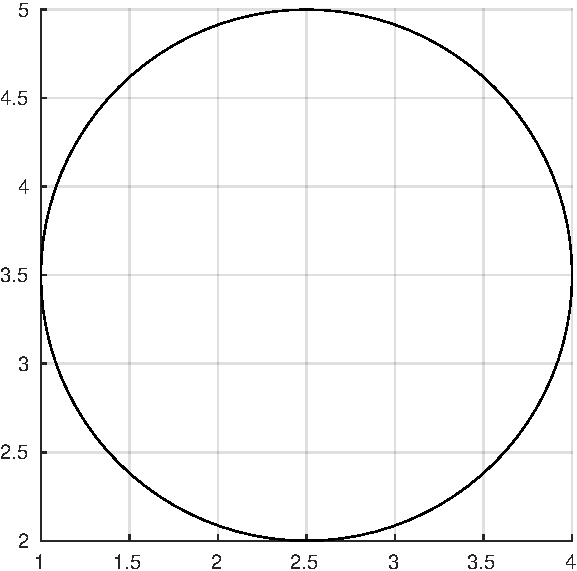
\includegraphics[width=0.5\textwidth]{Pics/exam-circle}
    \end{center}

    Hvernig mætti teikna þennan hring í Matlab? 

    Ath. að ásar hafa verið jafnaðir og rúðunet (e. \emph{grid}) hefur verið teiknað á myndina, skipanirnar að neðan sjá ekki um það.

    \begin{checkboxes}
    \CorrectChoice \verb|rectangle('Position', [1 2 3 3], 'Curvature', [1 1])|
    \choice \verb|rectangle('Position', [1 4 1 5], 'Curvature', [1 1])|
    \choice \verb|circle('Center', [2.5 3.5], 'Radius', 1.5)|
    \choice \verb|ellipse('Position', [1 2 3 3], 'Curvature', [0 0])|
    \choice \verb|rectangle('Position', [1 4 1 5], 'Curvature', [0 0])|
    \end{checkboxes}
\end{parts}

\newpage

\question Skrifið Matlab-skipanir (ein í hverjum lið) til að framkvæma eftirfarandi aðgerðir. Hver liður gefur eitt stig í stað tveggja sé hann rétt leystur en í meira en einni línu. Gerið ráð fyrir að skipanirnar í fyrri liðum hafi verið framkvæmdar rétt í seinni liðum.
\begin{parts}
\part[2] Búið til $3 \times 4$ fylkið \texttt{a}, sem inniheldur jafndreifðar slembiheiltölur á bilinu $[-2;3]$.
\vspace*{1.5cm}
\part[2] Búið til dálkvigurinn \texttt{b}, sem inniheldur summu hverrar línu í \texttt{a}.
\vspace*{1.5cm}
\part[2] Eyðið út dálki 1 í \texttt{a}, svo að \texttt{a} verði að $3 \times 3$ fylki.
\vspace*{1.5cm}
\part[2] Breytið \texttt{a} í $4 \times 3$ fylki með því að bæta neðst í það línuvigrinum \verb|[1, 2, 3]|, sem yrði þá lína 4 í \texttt{a}.
\vspace*{1.5cm}
\part[2] Búið til rökfylkið \texttt{odd}, sem inniheldur 1 þar sem tilsvarandi stak í \texttt{a} er oddatala en 0 annars.
\vspace*{3cm}
\end{parts}

\begin{solution}

\begin{minted}{matlab}
>> a = randi([-2 3], 3, 4);
>> b = sum(a')';
>> a(:, 1) = [];
>> a = [a;1:3];
>> odd = mod(a,2) == 1;
\end{minted}
\end{solution}

\newpage

\question[10] Skrifið Matlab-forrit sem les inn tölu frá notanda og skrifar út mynstrið sem sýnt er í sýnidæminu, með viðeigandi fjölda lína.

\begin{minted}{matlab}
>> square % Hér heitir forritið "square"
Hversu stór á ferningurinn að vera? 9
*########
**#######
***######
****#####
*****####
******###
*******##
********#
*********
\end{minted}

\begin{solution}

\begin{minted}{matlab}
n = input('Hversu stór á ferningurinn að vera? ');

for i = 1:n
    for j = 1:n
        if i >= j
            fprintf('*')
        else
            fprintf('#')
        end
    end
    fprintf('\n')
end
\end{minted}

\end{solution}

\newpage

\question[10] Tvíliðustuðlar (e. \emph{binomial coefficients}) koma víða við í stærðfræði. Tvíliðustuðullinn $C_{n,k}$ er skilgreindur fyrir hvert par af heiltölum $n$ og $k$ þar sem $n \geq k \geq 0$. Hann má reikna endurkvæmt út frá formúlunni $C_{n,k} = C_{n-1,k-1} + C_{n-1,k}$ með þeim upphafsskilyrðum að sé $k=0$ eða $k=n$ er $C_{n,k} = 1$.

Skrifið endurkvæma Matlab-fallið \texttt{binom} sem tekur inn gildi á $n$ og $k$ og skilar tilsvarandi tvíliðustuðli.

Fallið skal vinna með því að kalla á sjálft sig. Að hámarki helmingur stiga fæst fyrir lausn sem gerir það ekki.

Dæmi um mögulegar keyrslur fallsins:

\begin{minted}{matlab}
>> binom(1,0) % Eitt af upphafsskilyrðum
ans =
        1
>> binom(4,2) % Reiknað endurkvæmt
ans =
        6
\end{minted}

\begin{solution}
 
\begin{minted}[frame=lines]{matlab}
function p = pascalnumber(row,column)
if column == 0 || column == row
    p = 1;
else
    p = pascalnumber(row-1,column-1) + pascalnumber(row-1,column);    
end
end
\end{minted}

\end{solution}

\newpage

\question

\begin{parts}
\part[5] 

\begin{multicols}{2}
Gefin er skráin \texttt{gogn.txt}, sem er á sniði sem sjá má hér til hliðar. Skrifið Matlab-forrit sem les gögnin úr skránni. Setjið tölurnar í fyrri dálkinum í vigurinn \texttt{x} og tölurnar í seinni dálkinum í vigurinn \texttt{y}.

\begin{center}
\texttt{x 0.1; y 3.2\\
x 0.2; y 4.2\\
x 0.5; y 5.1\\
x 0.7; y 7.3\\
 ...   ...\\
}
\end{center}

\end{multicols}
\ifprintanswers
\else
\vspace{7cm}
\fi

\begin{solution}
\begin{minted}[frame=lines]{matlab}
fid = fopen('gogn.txt');
data = textscan(fid, 'x %f; y %f');
x = data{1};
y = data{2};
fclose(fid);
\end{minted}
\end{solution}

\part[5] Skrifið Matlab-skipanir sem teikna upp gagnapunkta með $x$-hnit geymd í vigrinum \texttt{x}, $y$-hnit geymd í vigrinum \texttt{y} ásamt feril þeirrar 3. stigs margliðu sem best nálgar punktana. Ferillinn skal teiknaður samfelldur, en gagnapunktarnir án línu á milli.

Gera má ráð fyrir að vigrarnir \texttt{x} og \texttt{y} hafi verið skilgreindir fyrirfram (t.d. með skipununum úr a-lið) og að þeir innihaldi a.m.k. 4 gagnapunkta.

\begin{solution}
\begin{minted}[frame=lines]{matlab}
equation = polyfit(x, y, 3);
equationX = linspace(min(x),max(x));
equationY = polyval(equation, equationX);
plot(equationX, equationY, x, y, 'k x')
\end{minted}
\end{solution}

\end{parts}

\newpage

\question
\begin{parts}
\part[5] Skrifið nafnlaust fall (e. \emph{anonymous function}) sem samsvarar eftirfarandi: 
\[f(x,y) = \frac{\sin \left(|x| + |y|\right)}{\sqrt{x^2+y^2}}\] 
Fallið skal geta tekið við vigurinntökum.

\vspace{2.5cm}

\part[5] Skrifið Matlab-skipanir sem sýna yfirborðsmynd (e. \emph{surface plot}) af fallinu í a)-lið frá -10 upp í 10 á bæði $x$-ásnum og $y$-ásnum með \texttt{winter} litavörpuninni. 

Gera má ráð fyrir að fallið $f$ hafi verið rétt skrifað í fyrri liðnum.

\end{parts}

\begin{solution}

\begin{minted}{matlab}
f = @(x,y) sin(abs(x) + abs(y))./(sqrt(x.^2 + y.^2));
x = linspace(-10,10); 
y = x; 
[X,Y] = meshgrid(x,y); 
Z = f(X,Y);
surf(X,Y,Z)
colormap('winter') eða % colormap winter
\end{minted}
\end{solution}

\newpage

\question[10] Skrifið Matlab-fallið \texttt{uniquesubstrings} sem tekur inn streng $s$ og tölu $n$ og skilar hólfavigri af öllum mismunandi hlutstrengjum strengsins $s$ af lengd $n$, án endurtekninga. Athugið að hlutstrengir mega skarast.

Gera má ráð fyrir að lengd $s$ sé stærri en $n$.

Dæmi um mögulega notkun fallsins:
\begin{minted}{matlab}
>> uniquesubstrings('bananar', 2)
ans = 
    'an'    'ar'    'ba'    'na'
\end{minted}

\begin{solution}
    
\begin{minted}[frame=lines]{matlab}
function uniques = uniquesubstrings(s, n)
m = length(s)-n+1;
subsstrings = cell(1,m);
for i = 1:m
    substrings{i} = s(i:i+n-1);
end
uniques = unique(substrings);
end
\end{minted}
   
\end{solution}

\newpage

\question[10] Leikurinn mylla (e. \emph{tic tac toe}) er flestum kunnuglegur. Spilarar skiptast á að fylla út í $3 \times 3$ rúðustrikað spilaborð með táknunum \texttt{x} og \texttt{o} þar til annar spilarinn hefur náð að fylla heila röð, heilan dálk eða heila hornalínu með tákni sínu, eða þar til ljóst er að hvorugur spilarinn nái markmiðinu.

Skrifið matlab-fallið \texttt{tictactoewinner} sem tekur inn $3 \times 3$ stafafylki sem táknar mylluborð (þar sem óútfylltir reitir eru táknaðir með biltákni). Ef annar spilarinn hefur unnið á því spilaborði skal fallið skila tákni þess spilara, annars skal það skila tómum streng.

Dæmi um keyrslu:

\begin{minted}{matlab}
>> tictactoewinner(['xoo';'ox ';' xx']) % x vann á hornalínu
ans =
    'x'
>> tictactoewinner(['xoo';'ox ';' x ']) % Enginn sigurvegari
ans =
    0×0 empty char array
>> 
\end{minted}

\begin{solution}

\begin{minted}{matlab}
function winner = tictactoewinner(board)

winner = '';
for i = 1:3
    if all(board(i,:) == board(i,1))
        winner = board(i,1);
    elseif all(board(:,i) == board(1,i))
        winner = board(1,i);
    end
end
if all(diag(board) == board(1,1))
    winner = board(1,1);
elseif all(diag(fliplr(board))) == board(1,end)
    winner = board(1,end);
end

end
\end{minted}
    
\end{solution}

\end{questions}
\end{document}